\chapter{Internet measurement with RIPE Atlas}
\label{sec:ripe_atlas}
\section*{Abstract}
Starting from this chapter, the center of our study is oriented to delay and path measurements, and how to make use of them in measurement-based interdomain \ac{TE}.
Same as volume statistics studied in Chapter~\ref{sec:pref_selec}, these measurements are readily available on client TE platforms.
However, we decided to switch to measurements conducted by RIPE Atlas, a measurement platform offering open data access to public, for the sake of reproducibility.

This decision is justified through a brief analysis on the elements of reproducibility and how RIPE Atlas satisfies them in design.
To facilitate the discussion in later chapter concerning measurement collection, we introduce succinctly the building blocks of RIPE Atlas, its measurement methods and how a particular measurement can be identified and retrieved.

RIPE Atlas is a great facilitator for a better understanding of the Internet, yet it is not without out problems. We studied the potential data quality issues stemmed from the platform itself, as well as those specific to the our study on inter-domain TE.
At the end of this chapter, we present a case study that inspires the remaining research in this thesis.
\clearpage

\section{Reproducibility}
\marginpar{Issue with previous dataset.}
We collected traffic volume and delay data from real client networks in Section~\ref{sec:pref_selec} and developed all the studies concerning prefix selection on that dataset.
Having access to real client data increases the credibility of the discoveries made in the study, and enhances the relevance of proposed schemes basing on these findings.
The other side of coin is that such private dataset hinder the reproducibility, a paramount feature in metrology researches.

\marginpar{What we talk about when we talk about reproducibility?}
The \acf{ACM} offers definition for various terms referring to different degrees of research repoducibility~\cite{acm}, ranging from repeating the same result by the same team to reproducing the same result with independent implementation of proposed methods or measurement system.
The way the measurement data is generated, stored and accessed is one of the key elements for all these degrees of reproducibility.

\marginpar{data generation}
Previous data from client network comes from measurements performed by proprietary commercial platforms~\cite{b6}.
By nature, it is against the fundamental benefit of the company to reveal the technical details on how measurements are done. Even permission of disclosure granted, we as research more often than not do not have enough space to include such technical details in publication.

\marginpar{data storage}
Since the collected data contain sensible information, e.g. the destination prefixes clients talked to, client IP addressing schemes, transit provider choices etc., they are required to remain on client owned platforms otherwise permission required. Due to capacity limitation and decreasing utility of old data, these measurements will not stay forever available on client servers. If measurements are allowed to be retrieved, we as researchers are then responsible for the storage of these data. Server clusters in research institution may offer temporary (available till graduation) storage infrastructure, yet researchers are responsible for the security of these data. Once data compromised, researchers may face serious legal consequences.

\marginpar{access to data}
Due to the sensitivity nature of data collected from client platforms, direct open access to the research community/public is not an option. Data anonymization is required. The process is not trivial as an appropriate balance is hard to hit. If not enough, some features of the client data can still be deduced and subject to unwanted exposure. If too much, the interpretation based on the anonymized data could become obscure and lack of credibility. Moreover, for better representativeness and statistical confidence, Internet measurement researches stress on large dataset over long period. This inevitably increases the size of dataset. Maintaining the access to these large dataset is clearly not without cost. However current publication reviewing process provides limited support on submitting voluminous supporting material without breaking the identity author/review anonymity~\cite{bajpai2017challenges}.

Bearing these considerations in mind, we look for measurement platforms alleviate the burden in measurement execution, storage and public access.

\section{RIPE Atlas for reproducibility}
RIPE Atlas is not the only Internet measurement platform that provides open data access~\cite{Bajpai2015}.
We justify this choice by first introducing RIPE Atlas. Then we summarize and highlight its features that qualify it as the best option for our research with comparison to alternative measurement platforms.

\subsection{Overview of RIPE Atlas}
\begin{figure}[!htb]
\centering
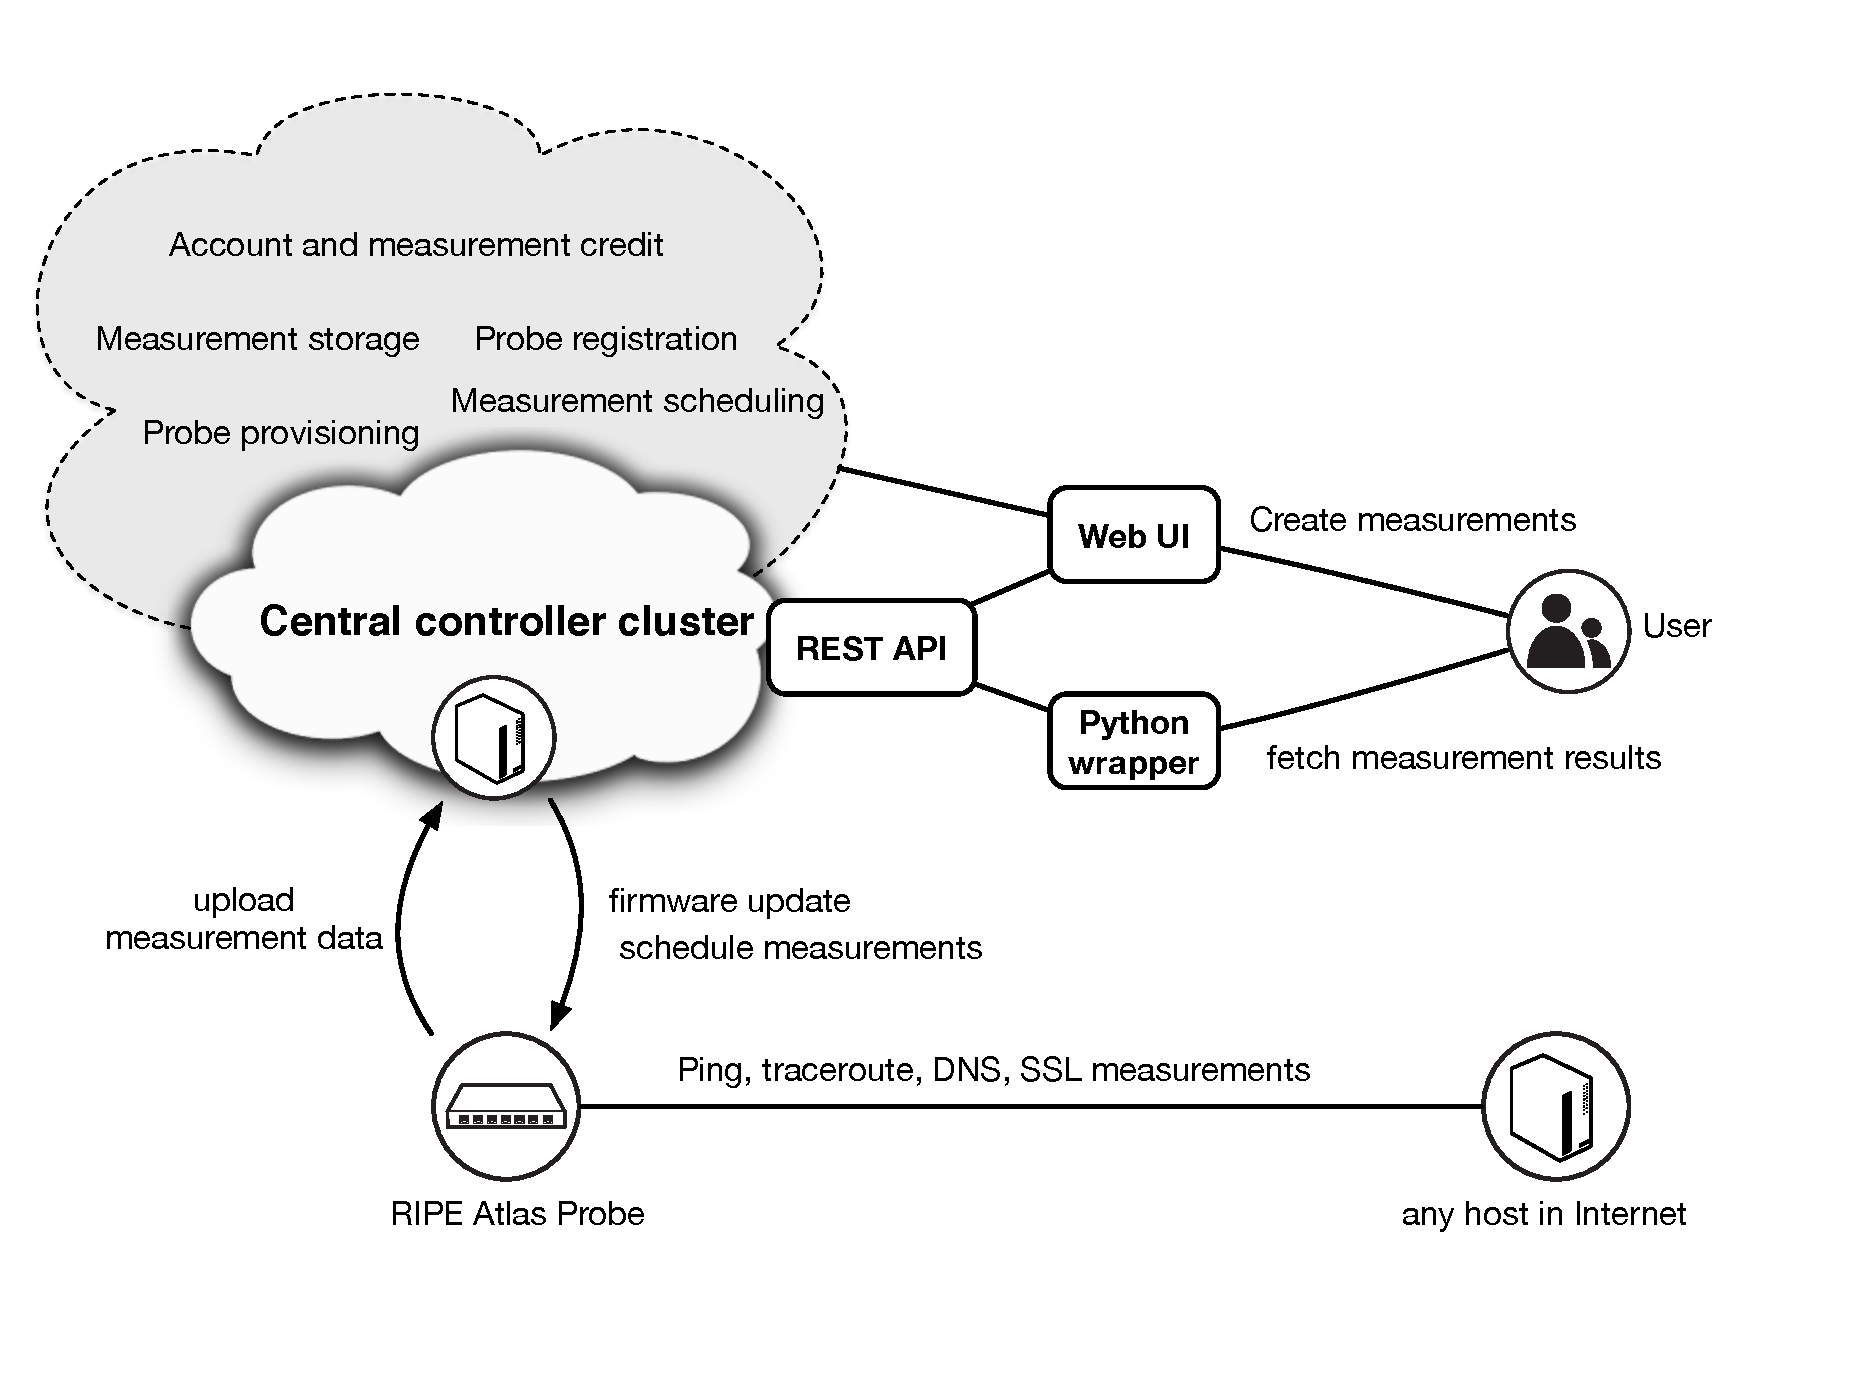
\includegraphics[width=\textwidth]{gfx/chap3/ripe_atlas_archi.pdf}
\caption{Building blocks of RIPE Atlas.}
\label{fig:ripe_atlas_archi}
\end{figure}

\acf{RIPE} Atlas is a measurement platform centrally managed by the European Internet register.
Fig.~\ref{fig:ripe_atlas_archi} sketches the architecture of the platform.
Probe are dedicated devices from which measurements are launched.
The operation system on the probes are tailored by RIPE engineers for Internet measurements~\cite{firmware}.
These probes are distributed either by RIPE or by RIPE Atlas Ambassador~\cite{ambassador} upon demand from anyone willing to host the probe and keep it online in his network.
As of this writing (July 11, 2017), 19448 probes have been sent out and 9854 of them remain active.
All these probes, hosted in 3511 IPv4 ASes and 1286 IPv6 ASes across 181 countries, can be commanded by a single platform user to measure any destination in the Internet.

As a platform user, one does not have to connect to all these probe by him/herself to 1) create specific measurements; 2) fetch measurement results. 
One only has to interface with RIPE to fulfill the above essential tasks along with other helpful functions such as measurement data visualization.
To that end, RIPE collects in quasi-realtime measurements from all the connected probes and stores them in its server clusters. Programming API~\cite{atlasapi} as well as human friendly Web sites are developed to facilitate the data operation of all kinds.

\subsection{Measurement types}
It is though not possible to run user specified measurement tools, e.g. nmnap~\cite{nmap}, scamper~\cite{luckie2010scamper} or bandwidth measurement tools, RIPE Atlas does support a wide range of standardized Internet measurements with configurable parameters: ping, traceroute, DNS, SSL.
Ping and traceroute measurement offer the Internet delay and path information required in measurement-based TE.

Another way of classifying the measurements is via the entity of measurement creator. As shown Fig.~\ref{fig:ripe_atlas_archi}, user of the platform (does not necessarily host probes) enjoys a great degree of 
liberty of specifying the destination and sources of supported measurements. These are \acf{UDM}. Once a user defines a measurement, the central controller clusters schedules it to corresponding probes and collects the results once the measurements started.
On the other hand, there exist another category of measurements defined by RIPE itself call built-in measurements~\cite{atlas}. These measurements are automatically executed by the probes themselves, with out need for controller commands. These measurements, originated from all probes, are mainly ping, traceroute and DNS measurements to DNS root servers and RIPE infrastructures.
In the later studies, we heavily rely on these built-in measurements given their world-wide footprint, super long history records (date back to the day one of each probe) and low additional measurement costs.

\subsection{Describe, identify and fetch measurements}
Besides measurement type specific parameters, such as the protocol type for traceroute, following three elements are as well fundamental describing a RIPE Atlas measurement: 1) participant probes; 2) the single measurement destination per measurement; 3) the time span of the measurement. 

Once a \ac{UDM} is created, it can be identified by an unique measurement ID. 
Each built-in measurement can as well be identified with a pre-assigned ID.
It is with this measurement ID, one learns the description, accesses data visualization provided by RIPE and eventually fetches the raw measurement results.
For example, with \url{https://atlas.ripe.net/measurements/3742863/#!openipmap}, one can have access to the path visualization of measurement $\#3742863$, where 100 probes word-wide are selected to perform one-time traceroute toward \url{www.sigcomm.org}. With \url{https://atlas.ripe.net/api/v2/measurements/3742863/results/?start=1462147200&stop=1462233599&format=json}, anyone can easily download the entire raw measurement records of this measurement.

\subsection{Advantages}
RIPE Atlas is a measurement platform designed to facilitate reproducible researches. RIPE take care of all the engineering challenges of 1) measurements execution from geographically distributed probes; 2) reliable and continuous data storage; 3) public access to data; 4) simple syntax for describing, identifying measurements; 5) well documented open-source programming tools for data manipulation.

The advantages of RIPE Atlas go beyond reproducibility. Compared to perfSONAR, PlanetLab and DIMES, probes of RIPE Atlas, with dedicated hardware for measurement task, are supposed to deliver measurements that better reflect the network character and are less impacted by probe local resource sharing issues~\footnote{perfSONAR: ~\url{https://www.perfsonar.net}; PlanetLab:~\url{https://www.planet-lab.org}; DIMES:~\url{http://www.netdimes.org}}.
Moreover, RIPE Atlas rapidly is gaining popularity among many non-academic networks, such as \ac{ISP}, \ac{CP} and \ac{IXP}, thanks to a wide range of monitoring applications hence enabled, to name a few, performance monitoring~\cite{latencymon, Rimondini2014}, anomalies detection~\cite{Fontugne2016, Padmanabhan, halo}, peering and IXP measurements~\cite{ixp, routeixp} etc. Increasing number of commercial networks host RIPE Atlas probes or anchors (a more powerful version of normal probe),   providing a much richer and realistic network profile from which measurements can be initiated, compared to other alternative options.

\section{Measurement quality}
We dedicate the discussion of this section to data quality, another key issue to metrology researches besides reproducibility. To begin with, we show that it is common to lose some datapoints for measurements scheduled at regular interval on RIPE Atlas. The temporal correlation between missing measurements and connection events are 
analyzed, in the pursuit of understanding reasons behind such missings.
To our surprise, a big part of measurements are lost while probes are connected.

Later on, with the RTT measurements from RIPE Atlas, we explore a data quality issue specific to interdomain TE. It deals with the fact that multiple measurements (potentially with different IP paths) could exist to quantify the transmission performance between two ASes. Are these measurements all alike? Which ones shall we use to make TE decisions?

\subsection{Missing measurements on RIPE Atlas}
\label{sec:miss_atlas}
Through previous studies~\cite{Holterbach2015a, Bajpai2015}, it is now known that load have obvious impacts on measurement precision and scheduling.
We focus on data completeness, another aspect of measurement quality that received less attention so far. Missing measurements can cause various undesired consequences. Apart from widening confidence interval of inference~\cite{Fontugne2016}, it requires in general methodological adaptations, e.g. in spectrum analysis~\cite{Babu2010, Luckie2014, shao2016}, otherwise biased estimation would be expected~\cite{Baraldi2010}.
%Therefore it is of relevance to question the nature of missing measurements.

One obvious reason of missing is that the probe is not running (properly), e.g. power off~\cite{schedule}.
As long as a probe is powered, it tries to maintain a connection to a controller to report measurements and receive assignments as shown in Fig.~\ref{fig:ripe_atlas_archi}. 
Therefore the probe connection activity provides a good indication of the probe availability, and is used in current investigation conducted by RIPE on probe OS stability~\cite{1look, 2look, 3look}.

In order to infer other possible causes, we compared the measurement timestamps with the moments probe connects to and disconnects from a Atlas controller.
If measurement missing coincides with the probe disconnection, chances are that the probe is dysfunctional during the missing. However, if measurements are lost while the probe is well connected, something `abnormal' should be expected, beyond the known probe OS issue.

\subsubsection{Data collection}
We observed the RIPE Atlas platform for one month, from 2016-06-01 to 2016-07-01 UTC.
All the v3 probes first connected before the beginning date (11613 of them) are considered.
Connection events (measurement ID 7000) and built-in Ping measurements to DNS b-root (measurement ID 1010), a highly available destination, are collected~\cite{built-in}. 
Controllers and the ping destination are not within the same network.
Controller logs the moments at which probes connects to and disconnects from it.
The built-in ping measurement is scheduled on every probe at 4min interval. 
10800 ping results are thus expected from each probe within the month.
7353 probes, out of the available 11613, had Ping measurements during this period.

\subsubsection{Missing at first glance}
\begin{figure}
\centering
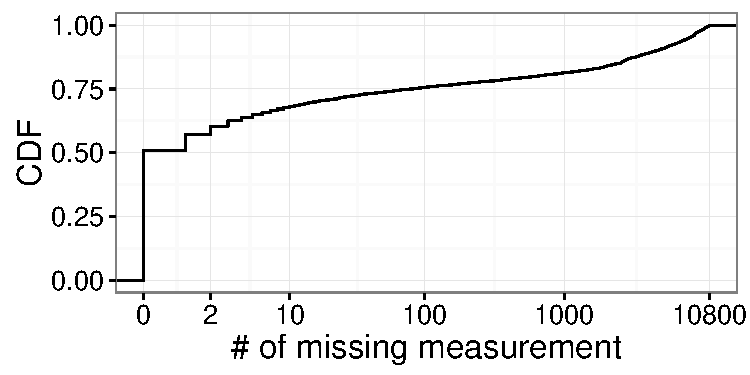
\includegraphics[width=0.7\textwidth]{gfx/chap3/missing_length_cdf.pdf}
\caption{CDF of total missing length per probe.}
\label{fig:miss_len}
\end{figure}
We deem that there are missing measurements when the time interval between two neighbouring measurement are much longer than the planned value. 
Such long gaps turn out to be very close to integer times of planned interval, as a cron-like mechanism is used to run measurements at regular interval and it retakes the previous phase after interruption~\cite{source, schedule}.
This character allows quantifying the length of missing segment by the number of measurements skipped.
4440 probes  (60.4\%) miss no more than 2 datapoints, which is totally legitimate, as random jitter is added to each single measurement to avoid synchronization among probes.
For the rest, the missing length spans a wide range according to Fig.~\ref{fig:miss_len}.
1358 (18.5\%) probes miss more than 10\% of the total measurements (i.e. 72 hours over a month).

\subsubsection{Cross missing measurement with connection events}

\begin{figure}[!htb]
\centering
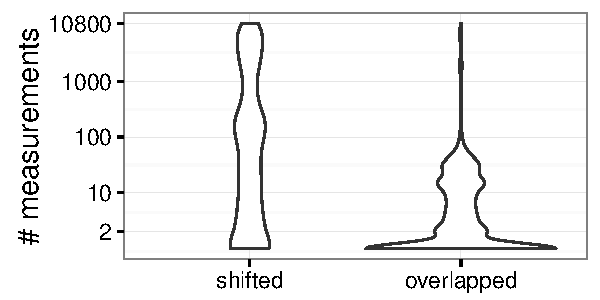
\includegraphics[width=0.6\textwidth]{gfx/chap3/len_by_ratio.pdf}
\caption{Missing length distribution.}
\label{fig:len_ratio}
\end{figure}

\marginpar{missing overlapped with connected period}
Several reasons may contribute to the disconnection of a probe to its controller: 1) probe not working (properly); 2) network issues preventing the connection; 3) controller not available, e.g. during maintenance~\cite{controller}. Meanwhile, the last two reasons shall not prevent a probe from performing built-in measurements, as the results can be unreachable or timeout, and be stored locally on the probe~\cite{usb}. 
That is to say, \textit{missing does not necessarily occur when probe is disconnected, but is unexpected while probe is connected.}

We count, for each missing segment, the number of missing measurements that occurred during a connected period.
We obtain the \textit{overlap ratio} by dividing this count by the length of missing segments. 
The distribution of overlap ratio is concentrated at the two ends, 0 and 1. 
For the convenience of illustration, we cut missing segments into two groups, one with overlap ratio $\leq0.5$, denoted as \textit{shifted}, the other with the rest, denoted as \textit{overlapped}.
Measurement missing that overlaps connected period is `unexpected'.

The two groups demonstrate different length distribution profiles, Fig.~\ref{fig:len_ratio}.
15391 missing segments are observed. 
10292 (66.87\%) missing segments are overlapped with connected period. 
They are mostly short in length. 5560 of them last no more than 2 measurements. 
One possible explanation is that these measurements are skipped due to scheduling or load issues~\cite{schedule, Holterbach2015a}.
Meanwhile, 2490 of them are equal to or longer than 1 hour, involving only 620 probes, for which we believe that the previous explanation hardly applies.
%% 620 probes ever have long overlapped missing segments, relatively a small portion.

Missing segments shifted from connected period are more likely to be long. This is possibly due to the v3 probe OS stability issue still under investigation. It is known to be responsible for long term probe disconnection and requires manual operation to recover the probe~\cite{usb, 1look, 2look, 3look}.

\begin{figure}[!htb]
\centering
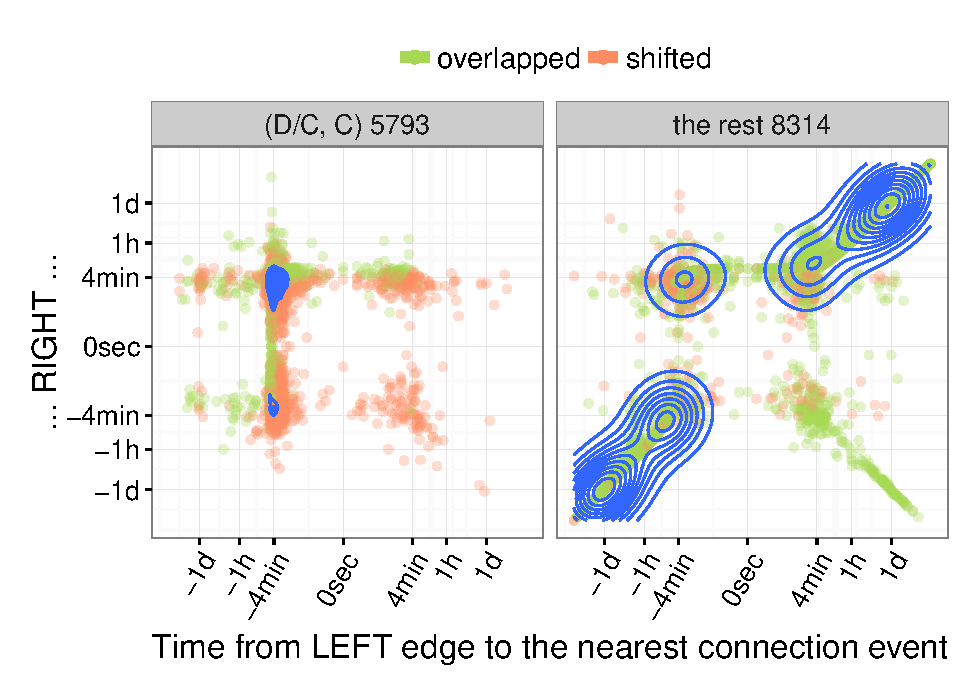
\includegraphics[width=0.98\textwidth]{gfx/chap3/all.pdf}
\caption{(D/C, C) stands for missing segments more closely correlated with disconnected period.
Number of concerned missing segments is given in the title. Negative time distance means the edge happens before the connection event and vice verse.}
\label{fig:all}
\end{figure}

\marginpar{temporal correlation between missing and connection events}
To obtain a subtler view, we seek to find out: when do measurements begin to be lost and when are they recovered? Are these moments close to connection events?

First, we define the \textit{left edge} as the last measurement before a period of measurement absence, and the \textit{right edge}, accordingly, the first measurement after recovery. 
We then calculate the time interval separating these edges and the closest connection events. We also identify the nature of these events, and mark `D/C' for disconnection, `C' for connection. 

1284 missing segments locate at the beginning or the end of the observation period. 
They are unavailable for this analysis as only one edge can be observed.
For the rest with both edges, 5793 missing segments' left edge is closer to a disconnection event and the right edge is closer to a connection event, according to Fig.~\ref{fig:all} sub-graph (D/C, C).
Judging from the density contour, last measurement most likely precedes disconnection by a Ping interval (4min), and recovery tends to take place 4 minute after the connection.
Such strong correlation with probe disconnected period indicates that probe dysfunction is probably the cause.

However, the beginning of such missing segments (D/C, C) can as well be dislocated from disconnection event.
At the left end of the graph, measurements are lost long before the disconnection, which we find `abnormal', even though the recovery is near connection.

To the right end, measurements only begin to be lost a long time after the probe is disconnected. One possible explanation is that measurements are first stored locally after disconnection from controller~\cite{usb}. Then new measurements are lost after local storage is full.

Contrary to the compact distribution in (D/C, C) sub-graph, the majority of the rest missing segments spreads along the time axis. 
The distances from left and right edge to connection events are highly correlated, suggesting that both left and right edges are on the same side of a same connection event.
We note that these measurements were mostly lost while probes were well connected, i.e. overlapped.

\subsubsection*{Wrap-up}
In our analysis covering a large number of probes over one month, only 60\% of v3 Atlas probes have complete measurements. Around $1/3$ missing segments appear to closely correlated to disconnected period. The probe OS stability issue might have contributed to such missings, as suggested by the heavy tail of the missing lengths.

However, the remaining $2/3$ of missings occurred while probes are connected. 
Half of them are no more than 2 measurements in length, and are thus likely to be caused by scheduling issues. However, around $25\%$ of this category lasts long($\geq 1h$). 
We reported the discovery to RIPE engineering team along with a specific case that they could started with.
The last reply from RIPE team confirmed  that the probe we mentioned in report had ``time synchronization issues''. To help advance the investigation, we share with RIPE team all the long missing segments identified. These exchanges can be found on the RIPE Atlas forum at \url{https://www.ripe.net/participate/mail/forum/ripe-atlas}, with tile ``Actual measurement interval much larger than planned''.

\subsection{Same AS path measured by different probes}
Whether the measured RTT mainly reflects the network characteristics of AS paths traversed real traffic is a data quality concern specific in the context of measurement-based interdomain TE.
It is simply because route selection function in Fig.~\ref{fig:archi} relies on path performance measurements as input, more details in Chapter~\ref{sec:cpt_rtt}.
However, RTT measurements might be `polluted' either by non-network factors, say host-local issues as CPU overload, or non-representative sub-AS level network issues can not be optimized with interdomain TE, say local congestion along the ASes traversed. 
However, none of these previous works~\cite{Goldenberg2004, Akella2008} on measurement based inter-domian TE has realized the importance of this problem.

This data quality issue gives rise to a series of questions: if we measure over a period of time a same AS path with multiple different RTT measurements toward different hosts in the destination AS, what will these RTT time series look like? Will they have similar characters? If not, how can we pick out the ones fit best for our TE uses?
We try to answer to these question by performing clustering over a such set of RTT time series, in the purpose of automatically revealing their inherent structures.

\subsubsection{Data collection}
We emulated such RTT measurements between two ASes, the local client AS (one host) and one destination AS (multiple hosts) with RIPE Atlas built-in measurements $\#1006$ and $\#5006$.
They are respectively IPv4 ping and traceroute measurements from all Atals probes to m.root-servers.net (202.12.27.33). 
Ping measurement is scheduled at 240sec interval, while traceroute at 1800sec.
120 RIPE Atlas probes within AS3215 are selected to construct our database.\footnote{The 120 probes are the same ones in user-defined measurement \#2427397 with open access to all.}
We assumed that all probes hit the same DNS root server clusters as the AS-level path toward the destination (m-root) is the same, since the only upstream AS for AS3215 is AS5511, the backbone of a French \ac{ISP}. Time window for the data collection ranges from 2015-09-28 10:00:00 UTC to 2015-09-29 12:00:00 UTC.

We cleaned the data collected, with following steps:
\begin{itemize}
\item Remove probes with unstable connection to the Atlas platform. (Short total length, multiple missing segments~\ref{sec:miss_atlas});
\item Remove probes suffering from obvious hardware or local network issues. (high packet loss, or error flag found in measurement results).
\end{itemize}

We then consider only 100 common probes in both ping and trace traces remained after cleaning.
All valid probes considered, the average hop number to the destination, m-root server, is 9. 
For the traceroute data set, we decided to concentrate on the first 3 hops (which should represent the access network). As a consequence, the traceroute data set are further cut into 3 parts, where each contains the RTT time-series till the corresponding hop.

To sum up, we fabricated four RTT time series data sets, on which we performed time series clustering:
\begin{itemize}
\item \texttt{pingData}, end-to-end RTT time series;
\item \texttt{traceData1}, RTT series till the first hop;
\item \texttt{traceData2}, RTT series till the second hop;
\item \texttt{traceData3}, RTT series till the third hop;
\end{itemize}

\subsubsection{Clustering RTT series in feature space}
Generally speaking, a time series clustering approach can be decomposed into three parts: data representation, distance measure and clustering algorithm~\cite{Aghabozorgi2015}. 
Due to its high dimension, time series is seldom used in its raw form, whence data representation.
Common approaches include dimension reduction~\cite{Elhamifar2013}, pattern extraction~\cite{Ulanova2015}, etc.
Distance measure quantifies the similarity/dissimilarity of two time series. Finally, clustering algorithm defines the procedure of grouping time series based the distances calculated on their data representation space.
For each of these components, multiple possibilities exist. However, it is not clear which one and which combinations of them could be the best fit to RTT measurements. 

\marginpar{data representation adopted}
In this section, we extracted a set of features listed below from each individual time-series and used in actual clustering. 
The advantage of such data representation is that it first largely reduces the data dimension. Thanks to that, data set is more suitable to classic partitioning clustering methods, like k-means and k-medoids (also known as PAM, partitioning around medoids)~\cite{Lin2003}.
Second, it is able to depict the data set from multiple aspects that are not evident with the raw form. 
%However, the clustering results could be biased by the selection of features.
Before clustering, each feature is z-normalized (zero mean and unit variance).
%so that result is not biased towards features with big value and high variance.
%%% At last I understood !!! Eureka. 

Following features are used in this work:
\begin{description}
\item[Power spectral density] is calculated using PyEgg~\cite{Bao2011} and cut into three bins, $(0, 1/12], (1/12, 1/6]$ and $(1/6, 1/2]$ of measurement frequency. Each of the bins individually functions as a feature.
\item[Sampling Entropy] proposed by Richman and Moorman~\cite{Richman2000} quantifies the regularity or predictability of a time series. In calculation~\cite{Bao2011}, we used an embed dimension of 2 and a tolerance of 15 msec.
\item[Number of changes] counts the number of times where the difference between two consecutive RTT measurements is greater than 15msec. %We did not use change detection methods that adapt to mean and deviation level of a window in the past, e.g. those based on z-score, for we assert that an absolute RTT change more than 15msec is significant, regardless of the mean and $std$ of an RTT trace. 
\item[Range] is the difference between the maximum and the minimum values of an RTT series.
\item[Mode] is the value most frequently present in a time-series.
\item[Mean], the first-order moment, describes the overall RTT level.
\item[Standard deviation] is derived from the second-order moment, describes how close measurements are to the mean.
\item[Skewness], the third-order moment, describes the lack of symmetry of RTT values observed around the center point of histogram, mode.
\item[Kurtosis], the fourth-order moment, describes whether the histogram of observations are peaked or flat relative to a normal distribution.
\end{description}
With RTT time series represented in the above feature space, we simply use euclidean distance to measure the distance between two RTT time series.

\begin{figure}[!htb]
    \centering
    \begin{subfigure}[b]{.7\textwidth}
	\centering
	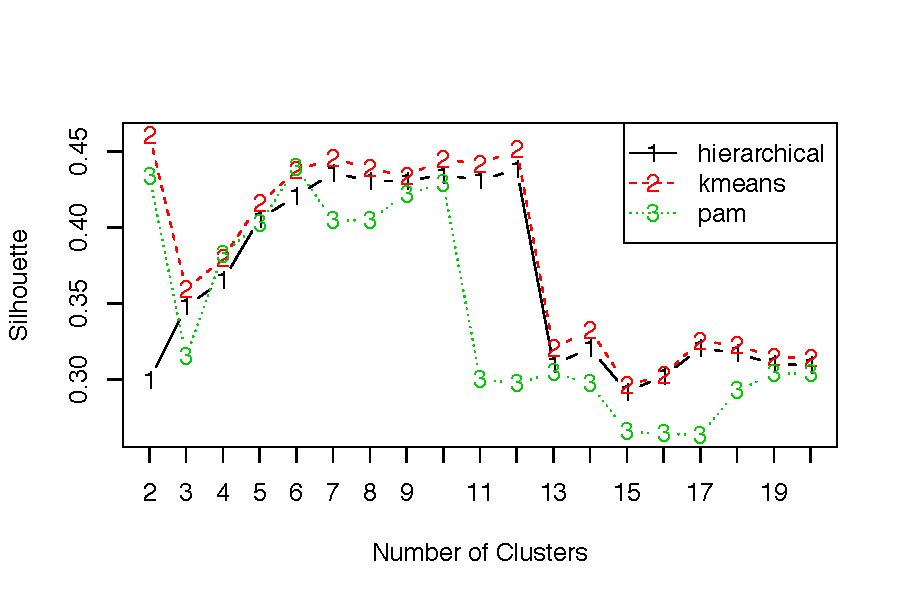
\includegraphics[width=\textwidth]{gfx/chap3/pingSil.pdf}
	\caption{\scriptsize \texttt{pingData}}
	\label{fig:pingSil}
	\end{subfigure}
	\begin{subfigure}[b]{.7\textwidth}
	\centering
	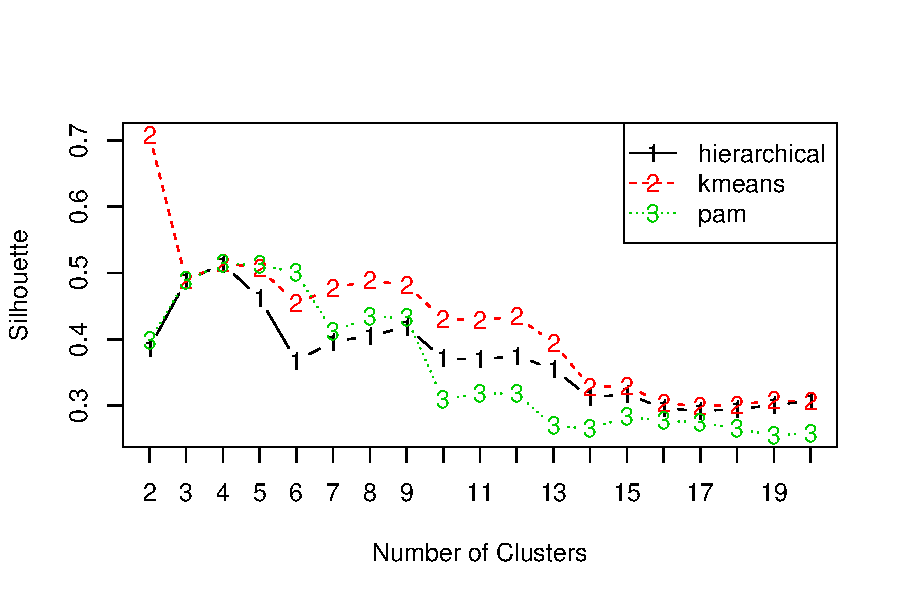
\includegraphics[width=\textwidth]{gfx/chap3/traceSil1.pdf}
	\caption{\scriptsize \texttt{traceData1}}
	\label{fig:traceSil1}
	\end{subfigure}
	\begin{subfigure}[b]{.7\textwidth}
	\centering
	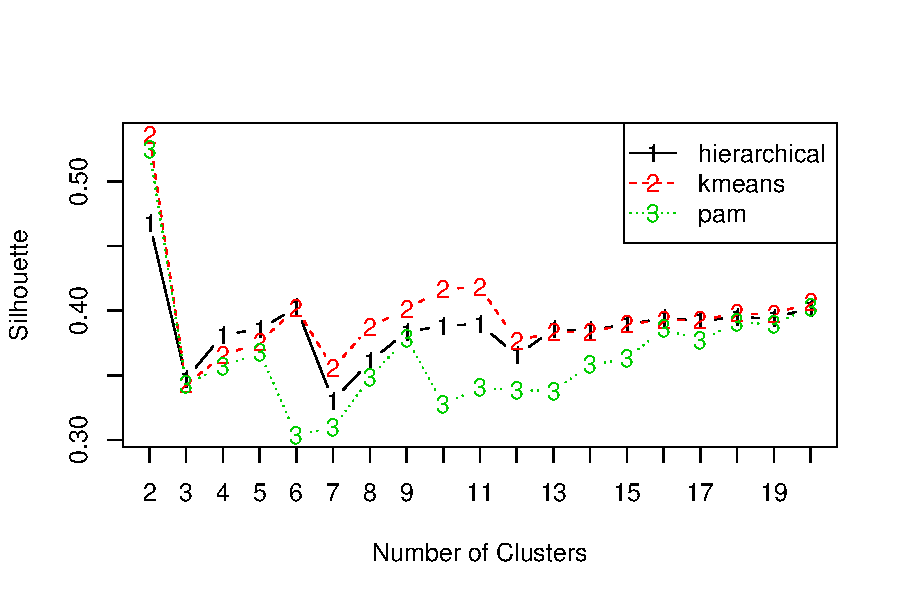
\includegraphics[width=\textwidth]{gfx/chap3/traceSil2.pdf}
	\caption{\scriptsize \texttt{traceData2}}
	\label{fig:traceSil2}
	\end{subfigure}
	\begin{subfigure}[b]{.7\textwidth}
	\centering
	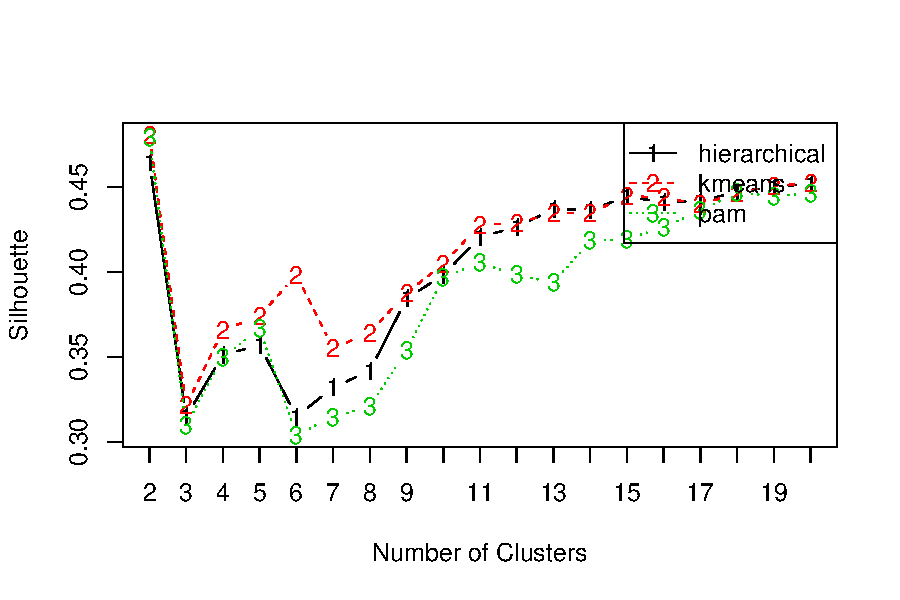
\includegraphics[width=\textwidth]{gfx/chap3/traceSil3.pdf}
	\caption{\scriptsize \texttt{traceData3}}
	\label{fig:traceSil3}
	\end{subfigure}
\caption{ASW (Average Silhouette Width) using different clustering algorithms when varying number of clusters.}
\label{fig:sil}
\end{figure}

\marginpar{Which cluster method is the most appropriate?}
Several clustering algorithms are available. 
In order to choose the one that fits best to our data set and decide the most appropriate cluster number, we use \acf{ASW}~\cite{Rousseeuw1987} to evaluate the quality of resulted clusters. 
It takes value in the range of $[-1,1]$. 
\ac{ASW} of a certain achieved cluster is a measure of how tightly all the data in the cluster are grouped together. 
While the \ac{ASW} over the entire dataset, is a measure of how appropriately the data has been clustered. For a single clustering method, we can find out what is the cluster number k that this algorithm is most confident of by picking the k offering the biggest \ac{ASW}. Across two different clustering algorithms, we could tell which one performs better by comparing the \ac{ASW} of resulted clusters, i.e. a better clustering result shall have a bigger \ac{ASW} value.

Following clustering algorithms are tested: hierarchical clustering with Ward linkage, k-means, \ac{PAM}.
Dataset-wide \ac{ASW} are visualized in Fig.~\ref{fig:sil}. We can see that for all the four data sets, k-means algorithm with $k=2$ offers relatively confident clustering results. 
Hence, such settings are used in the rest of the work.


\subsubsection{Clustering result interpretation}

\begin{table}[!htb]
\centering
\footnotesize
\setlength{\tabcolsep}{0.5em}
\begin{tabular}{l|ccc|ccc|ccc|ccc}
\toprule
\multirow{2}{*}{\# cls} & \multicolumn{3}{c|}{\texttt{pingData}} & \multicolumn{3}{c|}{\texttt{traceData1}} & \multicolumn{3}{c|}{\texttt{traceData2}} & \multicolumn{3}{c}{\texttt{traceData3}}\\
& size & dist. & AWS & size & dist. & AWS & size & dist. & AWS & size& dist. & AWS\\
\midrule
1 & 25 & 4.37 & 0.23 & 93 & 3.98 & -0.21 & 76 & 3.02 & 0.41 & 31 & 4.35 & 0.07\\
2 & 75 & 2.61 & 0.54 & 7  & 2.17 & 0.35  & 24 & 4.58 & 0.08 & 69 & 2.90 & 0.41\\ 
\midrule
AWS &\multicolumn{3}{c|}{0.46} & \multicolumn{3}{c|}{-0.17} & \multicolumn{3}{c|}{0.33} & \multicolumn{3}{c}{0.30}\\
\bottomrule
\end{tabular}
\caption{Summary of clusters characters on \texttt{PingData} feature space. Clusters are achieved from each corresponding dataset, while the statistics of clusters are computed with \texttt{PingData}.}
\label{tab:summary_cls}
\end{table}

\marginpar{How the two clusters are different from each other?}
Table~\ref{tab:summary_cls} provides several metrics describing the achieved clusters: size of cluster, intra-cluster distance, intra-cluster \ac{ASW}, and overall dataset-wide \ac{ASW} at the bottom.
Focusing on the column for \texttt{PingData}, we notice that two clusters of unbalanced size are obtained.
Cluster 2 is much larger in size, yet with smaller intra-cluster distance. 
In accordance, the cluster algorithm is more confident of this cluster than the other, as the cluster \ac{ASW} is much higher.
This indicates that the members within cluster 2 demonstrate strong common features and are thus more closely placed to each other in the feature space.

\begin{figure}[!htb]
\centering
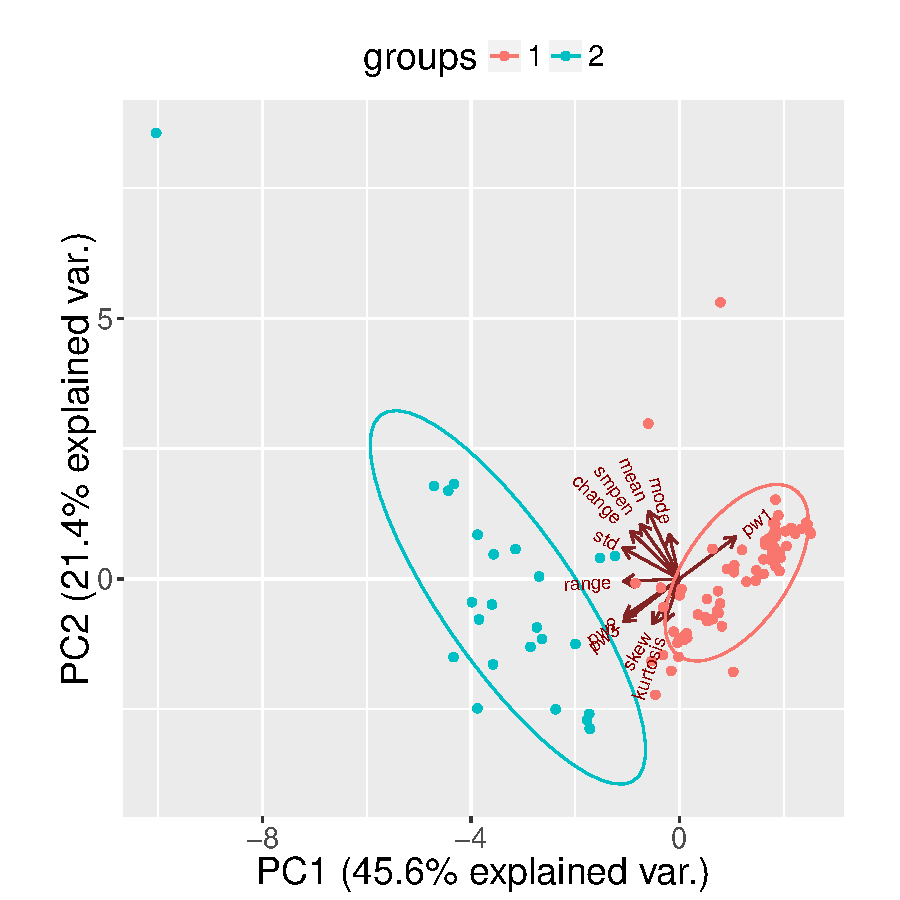
\includegraphics[width=.75\textwidth]{gfx/chap3/ping_pca_ping.pdf}
\caption{Projections of clusters on \ac{PCA} features, \texttt{PingData}.}
\label{fig:ping_pca}
\end{figure}

\marginpar{view from \ac{PCA} surface}
This ``guess'' can be straightforwardly observed from the projection of clusters on \acf{PCA} surface, shown in Fig.~\ref{fig:ping_pca}.
The contribution of each feature is as well indicated on the graph.
We notice that most of these points to different directions on the \ac{PCA} surface, suggesting that they are a comprehensive yet concise description of the date set.
As a consequence, no single feature takes dominant position in forming the clusters.
Still, tendency is that cluster 2 includes data points with little  changes, small entropy and small standard deviation. 

\begin{figure}[!htb]
    \centering
    \begin{subfigure}[b]{\textwidth}
	\centering
	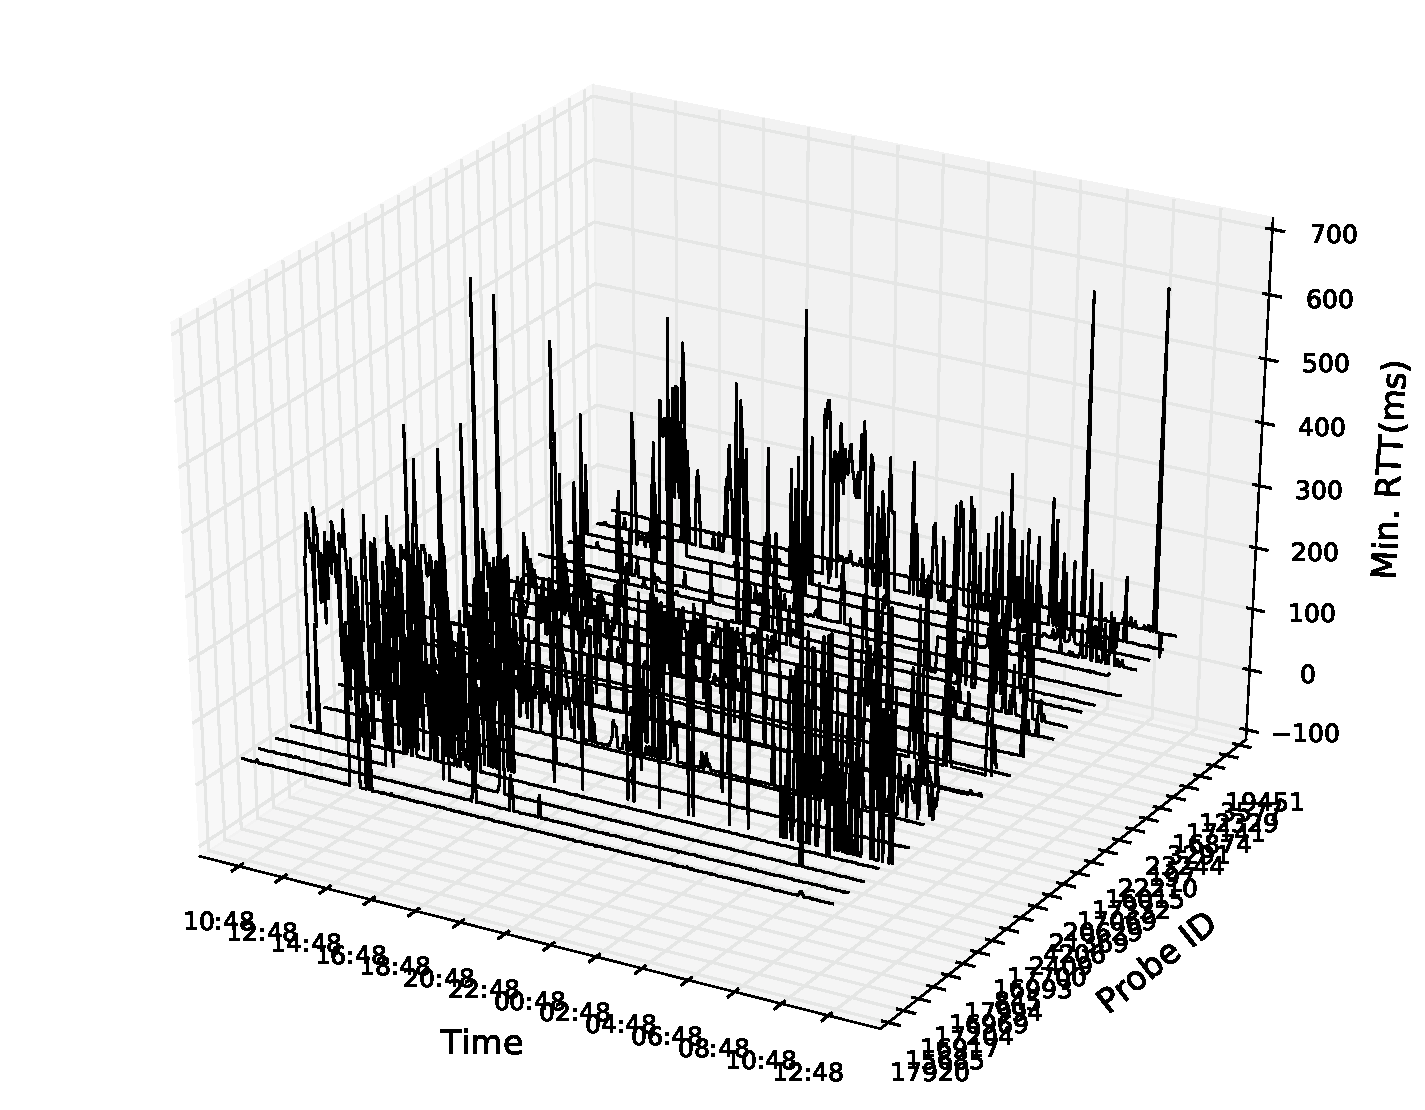
\includegraphics[width=\textwidth]{gfx/chap3/rtt3d_ping_cls1.pdf}
	\caption{cluster 1.}
	\label{fig:ping_cls1}
	\end{subfigure}
	\begin{subfigure}[b]{\textwidth}
	\centering
	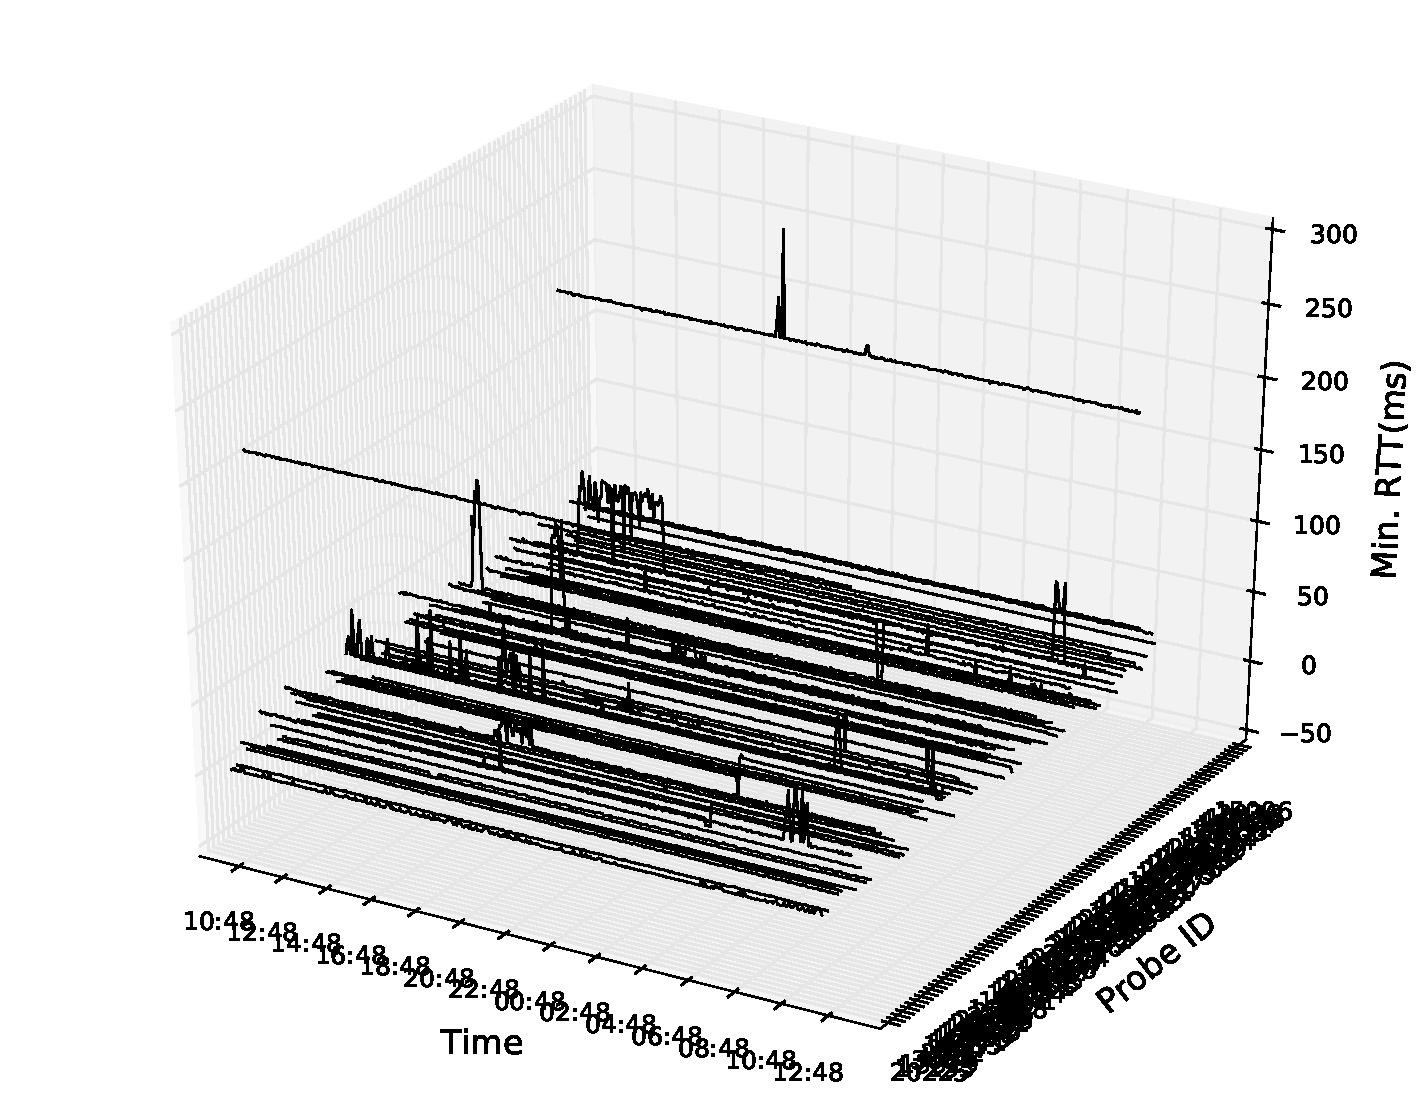
\includegraphics[width=\textwidth]{gfx/chap3/rtt3d_ping_cls2.pdf}
	\caption{cluster 2.}
	\label{fig:ping_cls2}
	\end{subfigure}
\caption{End-to-end RTT series of cluster members from \texttt{pingData} dataset.}
\label{fig:rtt_ping}
\end{figure}

\marginpar{view from RTT time series}
Fig.~\ref{fig:rtt_ping} plots the RTT time series of these two clusters. Cluster 2, as expected, contains mainly traces with only a few variations and spikes. 
On the other hand, cluster 1 is composed of traces with large variations.
This explains why the members of cluster 2 are more closely located to each other. 
It is because for a time-series to be smooth, there is only one form, while for it to be full of variations, there could be many possibilities.
%Let's also note that for smooth time-series (cluster 2), there is only one form, 
%while many different possible shapes can be observed in the other cluster.

\begin{figure}[!htb]
\centering
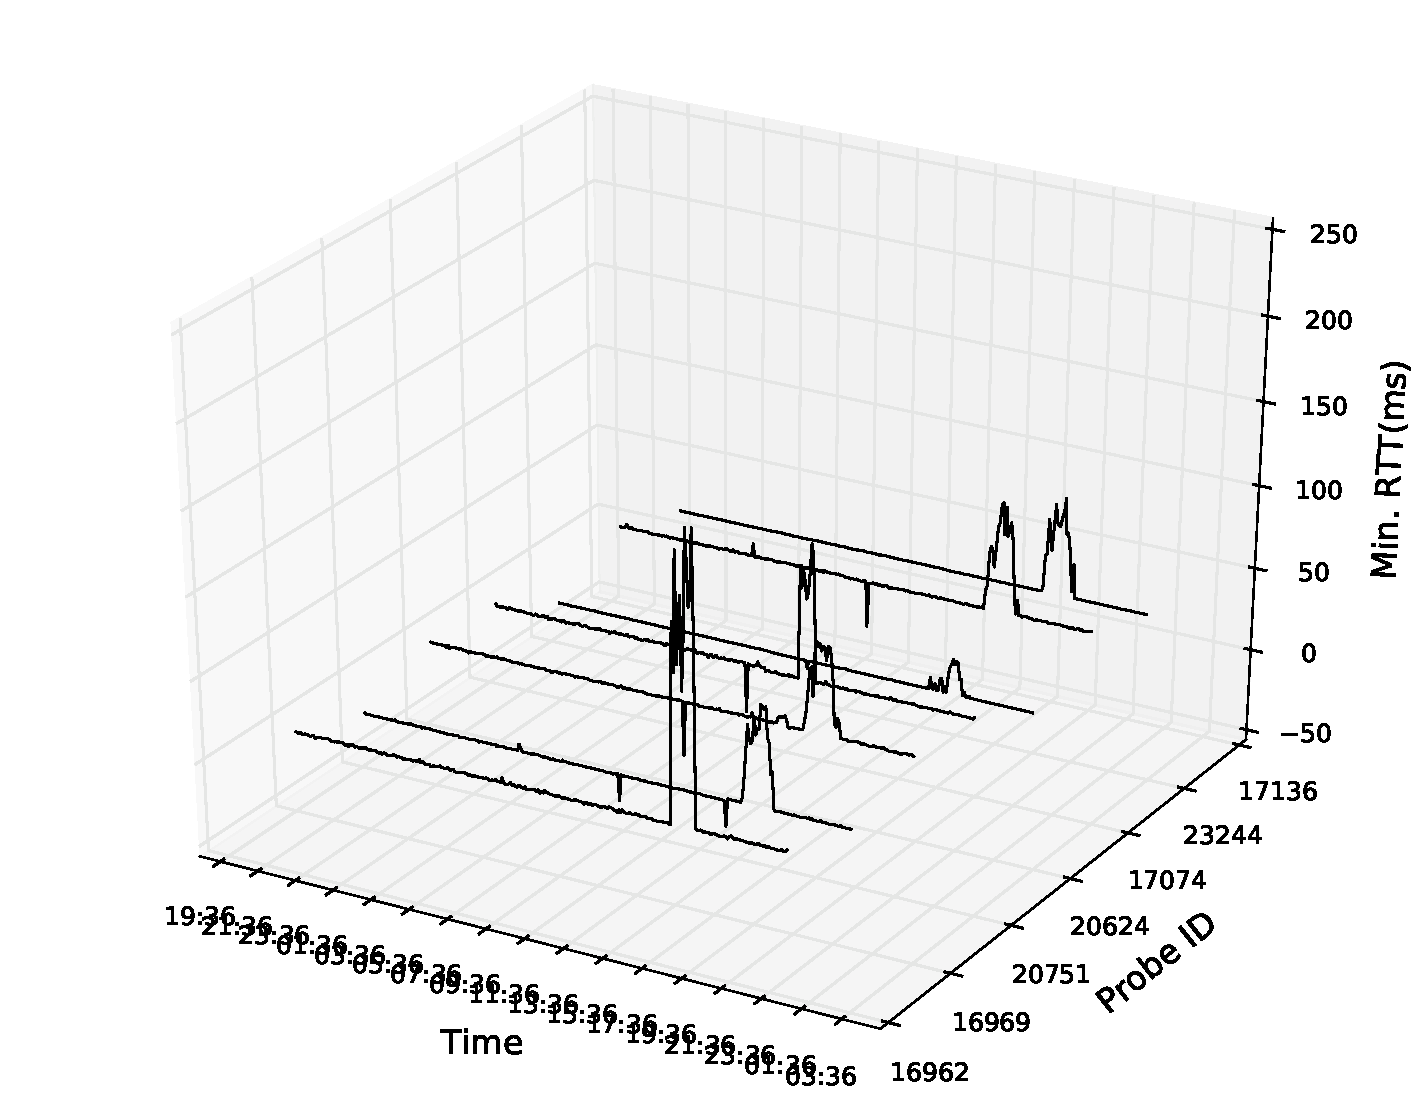
\includegraphics[width=.8\textwidth]{gfx/chap3/rtt3d_ft_pam_cls8.pdf}
\caption{One cluster achieved when $k=12$, \texttt{PingData}.}
\label{fig:cls8_k12}
\end{figure}

\marginpar{advantage of clustering with multiple features}
What is also worthy of noticing is that cluster 2 actually tolerates traces with a few spikes and variation of small amplitude. 
This is due to the advantage of using clustering instead of ranking with one single feature, which would also be viable to isolate ``noisy'' traces. 
For instance, we could rank the RTT traces by their entropy and assume top x traces are ``noisy'' ones. 
The shorting-coming of such approach is two-fold.
First, single feature might ``wrongly'' rank certain RTT time series. 
For example, entropy~\cite{Molina-Pico2011} and power spectral density are very sensitive to spikes. 
In networking uses, we believe that one or a few spikes in an RTT measurement shall not deteriorate an entire trace. 
Second, one has to define threshold values to deliberately separate data set into two or more parts. 
While with clustering, multiple features can be considered at same time. 
Plus, the most appropriate number of clusters changes automatically with the input and reveals the inherent structure of the data set. 
By setting a larger cluster number, one could achieve more fine-grained clustering results that convey subtler information. An example is given in Fig.~\ref{fig:cls8_k12}, where several traces of similar variation shape is grouped together.

\marginpar{interpretation in the context of interdomain TE}
The two clusters achieved are as well of relevance in interdomain TE. 
It shows that when measuring an AS-level path by probing multiple hosts in destination network, resulted RTT time series can take very different shapes. 
One possible explication is that the IP-level path toward certain hosts suffers from local problems.
If certain RTT variation is due to congestion on an inter-AS link, then it shall be shared by all the RTT time-series. If not shared, such RTT variation is probably related to local issues can not be avoided by changing an egress transit provider in sending out the traffic.
Therefore, when comparing multiple RTT time series between two ASes, the ones with fewer variations are supposed to be less impacted by these local conditions and give a more faithful view on the AS-level path performance.
One another advantage of using smoother RTT time series in choosing egress transit, is that resulted routes is supposed to be more stable. Fewer variations would actually trigger fewer route changes. 

\marginpar{take-away}
To summarize, when clustering RTT time-series in feature space, no specific assumption is imposed by the extracted features, yet we arrive at two clusters that tell noisy traces apart from smooth ones.
This reveals the inherent structure of the data set, that is for multiple RTT traces describing a common AS-level path, a majority of traces resembles each other and demonstrates least variations possible, while a handful of ``outliers'' may exist that contain diverse additional variations. 
Considering the source of our data, our assumption is that some of the RIPE Atlas probes are continuously suffering from local system or access network conditions. 
%%%TODO: caption of table 1, feature space, explanation
%%% What is "feature space". not defined sorry. 

\subsubsection{Where do the RTT variations come from?}

\begin{table}[!htb]
\centering
\footnotesize
\setlength{\tabcolsep}{0.5em}
\begin{tabular}{l|cc|cc|cc}
\toprule
\multirow{2}{*}{\texttt{pingData}} & \multicolumn{2}{c|}{\texttt{traceData1}} & \multicolumn{2}{c|}{\texttt{traceData2}} & \multicolumn{2}{c}{\texttt{traceData3}}\\
 &  1 & 2 & 1 & 2 & 1 & 2\\
\midrule
1 & 25 & 0 & 8 & 17 & 20 & 5 \\
2 & 68 & 7 & 68 & 7 & 11 & 64 \\
\bottomrule
\end{tabular}
\caption{Comparing cluster members resulted from different datasets. The number in each cell represent the number of common members share by the two clusters.}
\label{tab:comp_cls}
\end{table}

In this part, we tried to find out the origin of these additional RTT variations in cluster 1 of \texttt{PingData}, and their practical meanings in networking.
To this end, we clustered the RTT time-series of the first 3 hops extracted from traceroute measurements, and compared the cluster members to the ones obtained from end-to-end ping measurements in Table~\ref{tab:comp_cls}.

We observed that for \texttt{traceData2} (hop 2) and \texttt{traceData3} (hop 3), not only the cluster sizes arrived are in accordance to those from \texttt{pingData}, but also a majority of cluster members overlaps. 
That is to say, using RTT series till the 2nd hop or the 3rd hop, we ended up with similar clustering results as with end-to-end RTT series. 
This observation is further confirmed by Table~\ref{tab:summary_cls}, which calculates some statistic measures on \texttt{pingData} feature space for clusters resulted from each dataset. 
Clusters from \texttt{traceData1} have the poorest overall AWS indicating that its clusters are not a good fit for end-to-end RTT time series. 
However, clusters resulted from \texttt{traceData2} and \texttt{traceData3} seems to be quite OK on the feature space of \texttt{PingData}, as the overall AWS is not far away from that achieved with \texttt{PingData} itself.
%Considering that clustering on the feature space can indeed group RTT time-series by their level of variance, shown in Fig.~\ref{fig:rtt_ping} and Fig.~\ref{fig:ping_pca},
As clustering results on end-to-end RTT and on RTT towards the 
2nd and 3rd hop are highly similar, we are able to assume that most variations in the end-to-end RTT data set are expressed by the link between 1st and 2nd hop.

\begin{figure}[!htb]
\centering
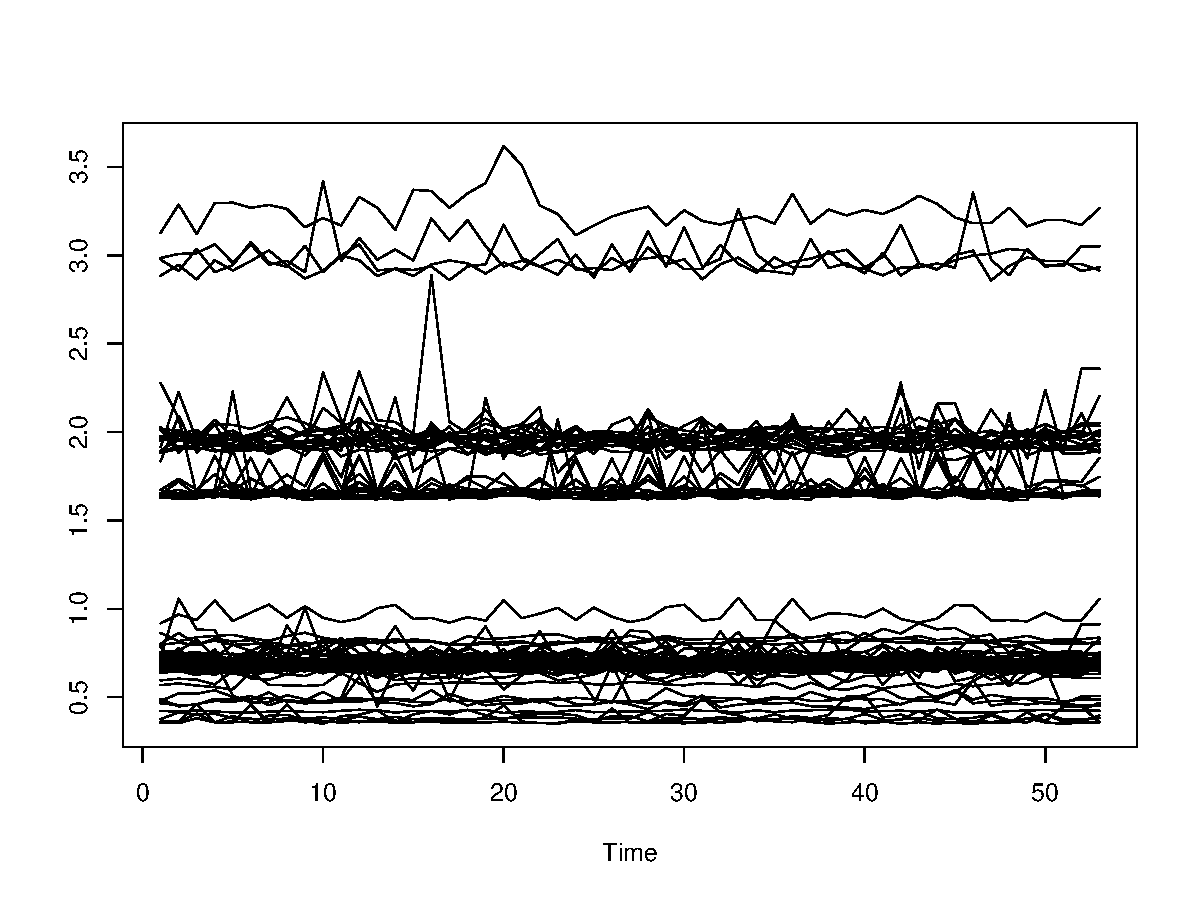
\includegraphics[width=.7\textwidth]{gfx/chap3/trace1_cls2_traceRTT.pdf}
\caption{RTT (in msec) till first hop. The first hop is assumed to be the hop till home router, yet three different baselines are observed. This might due to differences in connection methods, hardware and firmware versions of Atlas probe and ISP home router.}
\label{fig:trace1_traceRTT}
\end{figure}

In this specific case, where the probes involved are within the residential network of an ISP AS3215, the first hop probably arrives at the home router. This guess is indirectly confirmed by the observation that most traceroute records has \texttt{192.168.1.1} as the first hop address. As expected, RTT traces till the first hop are all generally pretty smooth according to Fig.~\ref{fig:trace1_traceRTT}. We manually searched second hop addresses, e.g. \texttt{80.10.127.143} in \url{https://db-ip.com/80.10.127.143}. Results returned show that they are all access equipment of the ISP.
It is thus logical to find most variation between the 1st hop (home router) and the 2nd hop (ISP access equipment), as it corresponds to the ISP access network.  

Such finding is of course not a huge surprise.% but rather a common sense among network engineers. 
However, it suggests that with our clustering method, we are able to get rid of RTT measures that undergo severe access network problems. 

\subsubsection*{Wrap-up}
In study, we date-mined RTT time series between two ASes. 
Such RTT traces emulates the measurements required in measurement-based interdomain TE, where multiple hosts in the destination ASes are probed to reveal the AS-path quality via certain transit provider.
We found out that RTT time series considered in this work demonstrate diverse variation shapes though one common AS path is measured.
It confirms the concern that RTT measurements need to be ``cleaned'' in inter-domain TE.
We clustered these RTT traces by extracting %a couple of 
several features. 
Resulted clusters successfully separate noisy traces from smooth ones according to human intuition and expertise.
Furthermore, we located the occurring location of most variations in end-to-end RTT measurements by applying presented clustering methods to the first hops of traceroute measurements.
Our results confirmed the common sense that most variations come from the access network.

\section{Synchronized RTT changes over different paths}
\label{sec:ripe_case_study}

A case, illustrated in Fig.~\ref{fig:trace1_traceRTT}, where multiple RTT measurements undergoing at the same time a similar shape RTT variation, intrigues us a lot. 
We wonder